\documentclass[../physical_computing.tex]{subfiles}

\begin{document}

\chapter{Lab Exercise 2 - Sequential Circuits}
\label{sec:appendix_3}

\section{Creating a project for a sequential circuit}
\label{sec:sequential}

Circuits implementing a sequence of instructions are called sequential. To define the sequence, and indeed to have any control over the evolution of our circuit with time, we need to implement a well controlled clock. The underlying circuitry was discussed in Chapter \ref{sec:registers}. The core element is a flip-flop whose gate input is connected to an oscillator.

Create a new VHDL project in a sub-directory of the \texttt{vivado\_projects} of your home directory. Copy the constraint file template into the project. Don't forget to check the box specifying that a copy of the constraint file should be made in the project. You can add the constraint file either when directed to specify constraints at the start of the process, or using the \texttt{add sources} button once the project is created. Don't forget to specify the correct FPGA part at the project creation stage. Remember to change the target language from Verilog to VHDL in the main pane of the project once it opens. 

Note that the name of the project can start with a number, so \texttt{32bit\_counter} is a perfectly valid project name. You can also start the names of VHDL source files with numbers. However, you cannot use a number for the name of an entity in a VHDL source file. This is worth mentioning, because if you decide to give a VHDL source file a name that starts with a number, the default name of the entity in the source file will be the same, and this will cause a syntax error. You can either not use numbers for VHDL source files, or you can rename the entity in the file once you have created it, in both the \texttt{entity} and \texttt{architecture} statements.

\section{32-bit Counter}
\label{sec:32bit}

The first project of Lab 2 is a 32 bit counter. The upper 16 bits of the counter will be converted to binary and displayed on the LEDs. You will need to edit your constraints file in the project and uncomment the lines defining the onboard clock based on the $\rm 100\,MHz$ MEMs oscillator attached to pin $\rm W5$. These lines are shown below, after the $//$ button in the main Vivado pane was used to remove a single \# comment character from the front of each line. Note that I have inserted a backslash character `\textbackslash' half way through the \texttt{create\_clock} statement. This is just so the text doesn't run off the page. The syntax of the constraint file is based on the Tcl language, and backslash is the line continuation character in Tcl. At any rate, later on the code seems to build and run fine with this modification. But, as I said, it's only there so I can fit the relevant lines of the constraint file within the page width of the book

\begin{minted}{tcl}
# Clock signal
set_property PACKAGE_PIN W5 [get_ports clk]
	set_property IOSTANDARD LVCMOS33 [get_ports clk]
	create_clock -add -name sys_clk_pin -period 10.00 \
	-waveform {0 5} [get_ports clk]
\end{minted}

To continue with the project you will need to use the `Add Sources' menu item in the `Flow Navigator' to add a VHDL source. Follow the guide from last week if you have forgotten what to do. When given the opportunity to specify ports, make sure there is an `in' port called clk to match the constraint file and an out port called led, which is a 16 bit wide bus. Note that the led elements will need un-commenting in the constraint file as well.

When your VHDL file appears, double click on it and take a look. The comments above the first library statement can be deleted - they are boilerplate intended for Engineers who need to record who wrote the code, the history of modifications, etc. Important in a large development team but not when you are writing your first small programs. This code is going to be using numeric data types, so you need to uncomment the IEEE numeric libraries that are by default commented out in the template. The first three lines of your code should look like this.

\begin{minted}{vhdl}
library IEEE;
use IEEE.STD_LOGIC_1164.ALL;
use IEEE.NUMERIC_STD.ALL;
\end{minted}

This has the effect of allowing logical and numeric data types within your program. Next follows the entity statement, where you specify the input and output ports for your part.

\begin{minted}{vhdl}
entity thirty_two_bit_counter is
    Port ( clk : in STD_LOGIC;
           led : out STD_LOGIC_VECTOR (15 downto 0));
end thirty_two_bit_counter;
\end{minted}

\section{Nodes and signals}
\label{sec:nodesandsignals}

Next comes the first portion of the architecture statement, where you describe the wiring inside the part. We immediately encounter some examples of nodes, which in VHDL are called signals.

\begin{minted}{vhdl}
architecture Behavioral of thirty_two_bit_counter is
  signal counter_d, counter_q : UNSIGNED (31 downto 0);
  signal counter_in_logic: STD_LOGIC_VECTOR (31 downto 0);
begin
-- rest of architecture specification code here
\end{minted}

Recall that the purposes of nodes is to supply points to which the ports of two or more gates, flip flops or other devices inside your circuit can attach. In this case, the two nodes on the upper line are for connecting to the $D$ and $Q$ ports of a flip-flop, and to connect to whatever operations are going to occur between $Q$ and $D$. These are of type UNSIGNED, which is the VHDL type for an unsigned integer. Our binary counter is going to count from zero up to $2^{32}-1$, then reset to zero automatically, because overflows are ignored. The other node, called \texttt{counter\_in\_logic} is needed because we need to cast the value of the counter from \texttt{UNSIGNED} to \texttt{STD\_LOGIC\_VECTOR} so that we can extract a subset of the bits and display them on the LEDs. There are two reasons why this is necessary. First, VHDL is a strongly typed language. There is no operator that can extract a subset of the bits of an integer. Second, recall that VHDL insists that the inputs and outputs of a device are represented by logical data types. So, even if our board had 32 LEDs and we could represent all the bits, the code would not compile if we were to try and wire the counter directly to the LED output.

\section{Processes}
\label{sec:processes}

The next part of the code is written to induce VHDL to connect some of the flip-flops on the board as registers. In order to do this, there must be an if statement, which you haven't met in VHDL, and this if statement must be inside a process. Since the outer of these statements is a process, let us start by explaining what processes are for.

The natural tendency in VHDL is for statements to correspond directly to wires that are connected in a circuit. Outside a process you cannot write two logically inconsistent statements. So, for example, if a node `myvar' is of data type \texttt{STD\_LOGIC}, then this code would not be allowed outside a process.

\begin{minted}{vhdl}
myvar <= '1';
myvar <= '0';
\end{minted}

This code literally instructs VHDL to connect the same node to logic level $1$, which is at least $\rm 2.0\,V$, and to logic level $0$, which is at most $\rm 0.8\,V$. This would cause a short circuit, and VHDL will not allow it. The purpose of processes is to permit data structures where there is a necessity for one instruction to supersede another one. In a process, if the same node is wired up several different ways in successive lines, then the last line takes precedence. So for example, this code is allowed

\begin{minted}{vhdl}
process begin
  myvar <= '0';
  myvar <= '1';
end process;
\end{minted}

The result would be that \texttt{myvar} would be wired to logic $1$, and not to logic $0$. What is the point of this construction? For a start, it is useful if you are going to use a conditional assignment, such as an if statement. For example, consider the following code

\begin{minted}{vhdl}
process(a) begin
  if (a='1') then
    myvar <= '0'; 
  else
    myvar <= '1';
  end if;
end process;
\end{minted}

If the node or port \texttt{a} is in logical state $1$, then \texttt{myvar} is wired to $0$, otherwise \texttt{myvar} is wired to $1$. The outcome depends on the state of \texttt{a}, and therefore the node or port \texttt{a} is included in the dependency list. The dependency list is a comma separated list of nodes or ports (I could say variables, but I'm trying to help you to avoid confusing hardware description languages and high level languages like PYTHON), in round brackets next to the process statement. Any nodes or ports whose value affects the outcome of the statements in the process is included in this list. You can see why conditionals like if...then...else are always wrapped in a process statement in VHDL. Their effect is to set the value of a node or port different ways depending on some other condition. We will meet other conditional statements later. 

Note also that, bearing in mind the earlier point about the last statement taking precedence, the following code is equivalent to the conditional example above

\begin{minted}{vhdl}
process(a) begin
  myvar <= '1';
  if (a='1') then
    myvar <= '0'; 
  end if;
end process;
\end{minted}

Here the first assignment of \texttt{myvar} as $1$ can be though of as a default. However, if it turns out that \texttt{a} is $1$, then the later assignment of \texttt{myvar} to $0$ supersedes the default. I think this way of using if...then conditionals is good practice, because if you set a default assignment for a node or port inside the process before the conditional, then the node or port is assigned to some value, whatever happens with the conditional. In VHDL, where it is crucial to avoid leaving hanging wires connected to nothing, the existence of a default for all nodes or ports is an important protection against hard-to-diagnose faults.

Now, consider the process and conditional statement that follows next in the code for the 32 bit counter.

\begin{minted}{vhdl}
  process(clk, counter_d) begin
    if(clk'event and clk='1') then
      counter_q <= counter_d;
    end if;
  end process;
\end{minted}

This is a special combination of a process and a conditional that is used specifically to set up memory registers. First, note that the outcome of the code depends on \texttt{clk} because it is used in the if...then statement. Also, the assignment of \texttt{counter\_q} depends on the state of \texttt{counter\_d}. Hence both \texttt{clk} are in the dependency list. Second, note the special purpose syntax inside the if statement. The first part, \texttt{clk'event} is a special instruction to look for edges in the \texttt{clk} port, times when the \texttt{clk} port is transitioning between states. The second part of the conditional checks that the value of \texttt{clk} after the transition is detected is $1$. The combination of these two conditionals is enough to induce VHDL to wire \texttt{clk} to the gate port of a flip-flop, since this is the only circuit element on the chip that can detect edges.

Since the hardware device being used is a flip-flop, we know that the only thing it can do is copy the value of its input, or $D$ port, to its output, or register, or $Q$ port, so the contents of this if...then statement have the effect of ensuring that 32 single bit flip-flops will have their input $D$ ports connected to the 32 bits of \texttt{counter\_d}, and their output $Q$ ports connected to the 32 bits of \texttt{counter\_q}. When rising clock edges appear, a momentary snapshot will be taken of the state of \texttt{counter\_d}, and copied to \texttt{counter\_q}, where it will remain persistent until the next rising clock edge.

Any number of register updating statements can be included in this special purpose process and conditional statement. But, no other operations should be put in this process! This is because the flip flop copy operation can happen almost instantaneously on the detection of an edge in the gate port, but all other operations, such as logical or arithmetical operations, take too long to be implemented on the clock edge like this. If you have other operations to perform, put them in a separate process.

Another good rule of thumb is that only inside this special process should you use the \texttt{d} port of a flip flop as the input on the right of the $<=$ operator, and the \texttt{q} port of a flip flop as the output on the left of the $<=$ operator. Outside this special process, you should always be setting the \texttt{d}, or input port, based on the value of the \texttt{q}, or output port. This means that all the time consuming operations have $\rm 10\,ns$ for their outputs to settle; the only operations that need to happen much faster are the copies inside the flip-flops, and these are fast by design.

\section{Counting}
\label{sec:counting}

To actually count upwards, we will use the $+$ operator, which implements binary addition on all the integer data types we will use in the course. Note that $+$ just adds binary sequences. The input and the output should have the same number of bits, and any overflows will be discarded. The code to implement the counting is very simple

\begin{minted}{vhdl}
counter_d <= counter_q + 1; 
\end{minted}

Since \texttt{counter\_q} is the currently stored value of the counter, and will remain static for $\rm 10\,ns$ between rising clock edges, all this statement does is ensure that the appropriate logic is in place between the node \texttt{counter\_q} at its input and the node \texttt{counter\_d} at its output such that \texttt{counter\_d} is one greater than \texttt{counter\_q}. At the next rising edge in \texttt{clk}, \texttt{counter\_d} is copied to \texttt{counter\_q} incrementing its value by $1$ and the cycle continues.

\section{Casting and selecting a subset of bits}
\label{sec:castandsubset}

The next two lines introduce us to casting and a further operation on logical data types, the selection of a subset of bits. 

\begin{minted}{vhdl}
  counter_in_logic <= std_logic_vector(counter_q);
  led <= counter_in_logic(31 downto 16);
\end{minted}

Note that since these lines are outside any process or conditional construction, they represent permanent wires between nodes and ports. In the upper line, the node \texttt{counter\_in\_logic} is connected to the output of a cast operation, with the currently stored value of the counter at the input. The cast operation is necessary because VHDL is a strongly typed language. You need to specify exactly what data type each node or port has. We want a node of the \texttt{STD\_LOGIC\_VECTOR} type with the same bus width as the 
counter, so we employ the \texttt{std\_logic\_vector()} operator, which casts a node or port into the \texttt{std\_logic\_vector} data type. In the lower line, we use the \texttt{31 downto 16} construct to select a subset of the bits in \texttt{counter\_in\_logic} to assign to the 16 \texttt{led} ports.

Lastly we must end the process, with 
\begin{minted}{vhdl}
  end Behavioural;
\end{minted}

Type in the code carefully, making sure you understand the concepts as you do so, as this code contains several new concepts. Ask myself or Mitch if you are unsure about anything. Then, run synthesis, implementation, and bitstream build in turn. At each stage, there may be errors or critical warnings - if the build fails you can check for these in the Messages tab of the lower pane. Once you have built your bitstream, follow the same procedure as last week to attach your board, launch the hardware server in a terminal window, open the hardware manager, connect it, program the board, and see if the lights count in binary.

\section{Gating your counter with a pushbutton}
\label{sec:buttons}

Let us next make a counter that only counts up when you have a pushbutton pressed, and stores the previously attained value when the counter is released, starting to count from that same value when the pushbutton is pressed again.

Close the hardware manager then use the \texttt{File->Project->Save As} option to save the project as a new name,
say \texttt{gated\_counter}. Make sure the directory of the new  \texttt{gated\_counter} project is in a subdirectory of \texttt{vivado\_projects}. There is no need to include run results in the new project, although it does no harm if you do.

Open up the constraint file, and scroll down until you find the lines referring to Buttons. There should be five sets of two line entries, each referring to one of the cluster of five pushbuttons arranged as 
central, up, left, right, down. Uncomment the two lines referring to the central button, then save the modified constraint file.

\section{Conditional assignments}
\label{sec:conditionalassignments}

We have already discussed if...then statements and stated that these have to be inside process statements. It turns out that there is one type of conditional which operates slightly differently, and as a consequence should never be inside a process. These are called
conditional assignments. Here is an example of a conditional assignment. In this case c is a 2 bit \texttt{std\_logic\_vector} and $a$ and $b$ are 32 bit signed integers.

\begin{minted}{vhdl}
  a <= b+1 when c="01" else
       b+10 when c="10" else
       b+100 when c="11" else
       b;
\end{minted}

Note the defining feature of conditional assignments, that the conditional exhausts all the possibilities for the controlling logic. In this case, a 2 bit parallel bus can only take the four values $B00$, $B01$, $B10$ and $B11$. The code specifies an outcome in each of those eventualities. In fact, this code is somewhat overengineered since the last else means that there is a default, which covers all eventualities other than those above. It is good practice always to include a default in conditional assignments.

Using this new construct, you should be able to modify the line
\begin{minted}{vhdl}
  counter_d <= counter_q + 1; 
\end{minted}
so that the effect is the one desired in this project - that when the pushbutton is pressed (this will make the corresponding port logic $1$), the counter continues to count up, but when the button is released, the count will stop and retain its value. Try and get this working without more detailed instructions.

\section{Counting button pushes}
\label{sec:pushbuttoncounter}

Now we are ready to try something significantly more challenging. Consider the humble pushbutton. Even if you press it for as short a time as you physically can, the duration of that press is going to be many thousands of $\rm 10\,ns$ clock cycles, as you can verify by watching the LEDs when you push the button as briefly as you can in the previous project. Given that, how do we build a code that increments a counter by exactly one every time a button is pressed?

Let's take a first guess at how to handle this task. Let us build a detector for changes of button state from zero to 1. After all, you might think that when you press a button it may stay in state $1$ for a long time, but maybe it only transitions from $0$ to $1$ once. Couldn't we use this to achieve our goal?

To try this idea, create a one bit register called \texttt{bstore}. This should have an input and an output node just like the counter register, and it should be implemented with a flip flop in just the same way. Connect the input node to the button. You can detect edges by comparing the current button state to the output node, which after all represents the button state last clock cycle. If the current button state is $1$ and the bstore output is $0$, this means that the button has just changed state from $0$ to $1$. If this is true, then increment the counter. Otherwise, leave the counter in its previous state.

See if you can get this working, and see if it works as well as you wanted it to, or if there are problems. If there are problems, then try to work out what is causing those problems. Here are a couple of hints. The register copy from \texttt{d} to \texttt{q} for bstore can be in the same process and if...then statement as that for the counter. You can reduce the number of bits in the counter from 32 to 16 and put all of them on the LEDs. You will no longer need the \texttt{counter\_in\_logic} node as you can cast \texttt{counter\_q} directly to the \texttt{led} outputs. Another hit is that conditional assignments can have logical combinations of several conditions after the \texttt{when} keyword and before the \texttt{else}. Finally, don't forget to modify the dependency list for the register to include \texttt{bstore\_d}.

\section{Bouncing buttons}
\label{sec:bounce}

If you play with your button-triggered counter for a while, you will probably find that, though most of the time it works fine, occasionally there will be one of two effects. The first effect you will sometimes see is that you will press the button once, but the count will increment by more than one unit. The second effect you will see sometimes is that there will be one or more counts at the moment you release the button. These problems are caused by the physical structure of the button itself. Figure \ref{fig:button} is a slightly exaggerated illustration of the problem.

\begin{figure}[htbp]
    \centering
    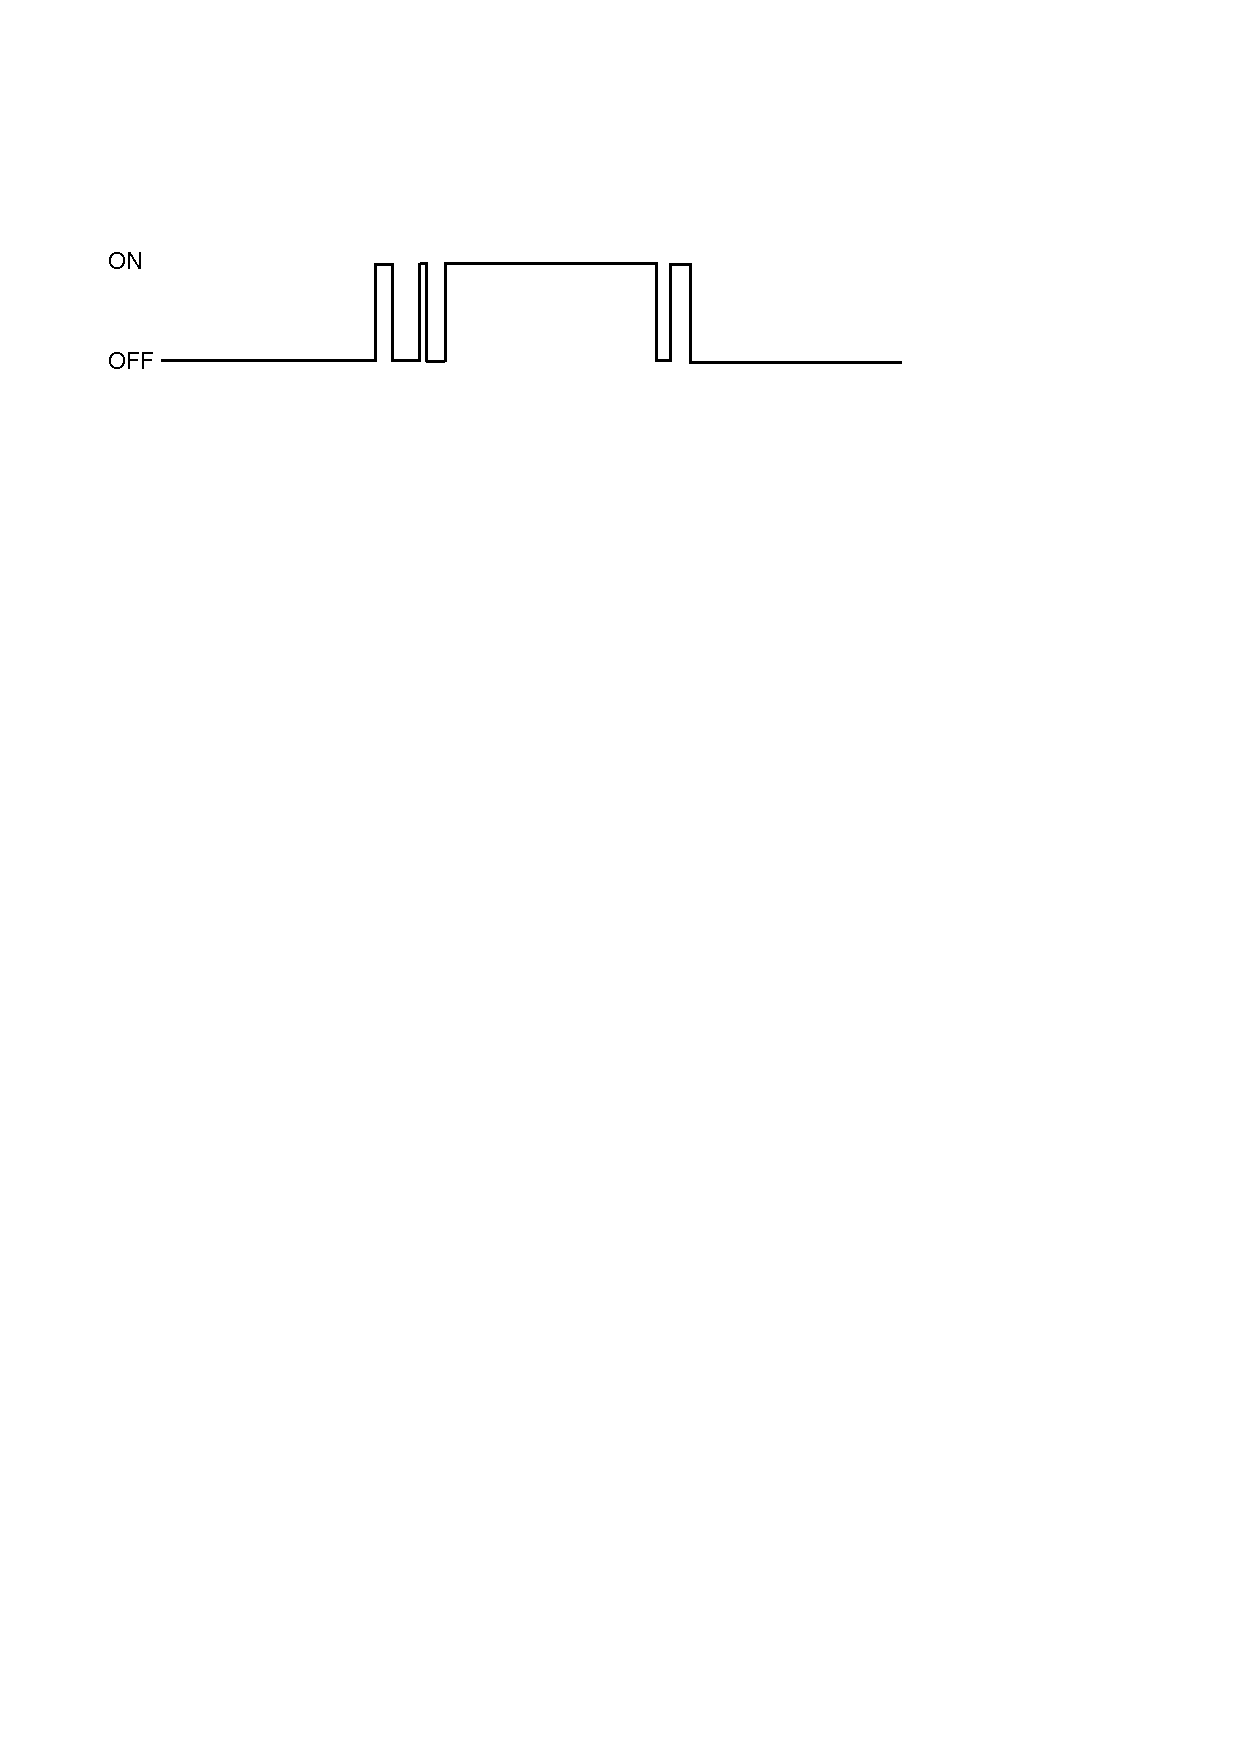
\includegraphics[width=0.5\textwidth]{figures/button.pdf}
    \caption{The bounce effect in a pushbutton.}
    \label{fig:button}
\end{figure}

The button is not mechanically perfect, and now and again, both at the pressing of the button, and the release, there are multiple state changes. This effect is called 'bounce' in engineering, and mechanisms to prevent it are called debouncing circuits. As our final project today, and the most challenging of them, we will think about how to make a debouncing circuit for our pushbutton.

There are in fact several ways to do it, and the better and clearer ones require programming constructs we have not studied yet, such as state machines. However, with what we already have we can try and make a button debouncer.

The first thing is to recognise that we are most of the way there. Our buttons appear to be of high enough quality, that the number of bounces is rarely more than one, and usually zero. A good question is, what makes multiple switches of state a bounce? The answer is that the multiple switches have to occur within a short time interval. What we want in a debouncer is a way of ignoring further changes of state that occur less than a certain short amount of time after an initial change of state is detected. As can be seen from Figure \ref{fig:button}, the same effect happens both on press and release, so this mechanism should be triggered both on the detection of a transition from $0$ to $1$ when the button is pressed, and on the detection of a transition from $1$ to $0$ when it is released. 

One way to implement this is with a second counter. We have one counter that is now just counting button presses. This counter needs to carry on doing its job. We are going to need a second counter that counts driven by the clock, as it was before in the very first project. However, it only needs to start counting up when a change of button state is detected. Let's say this counter is zero initially and the button is unpressed. Now our current mechanism detects a change of button state from $0$ to $1$. This increments the counter. It is no longer at zero. Let's say the next value of the counter depends on its current value. If the counter is at zero and no change of button state has been detected, the counter stays at zero. If the counter is at zero and a change of button state has been detected, the counter increments. If the counter is anything other than zero, it increments anyway, no matter what the state of the button. Thus, the counter keeps on counting up. Once the counter reaches its maximum capacity, it naturally resets to zero, at which point we're back to the zero state. Crucially, the counter not being zero implies that we are within a time interval, settable by a judicious choice of the number of bits in the counting variable. Only when a change of button state from 0 to 1 is detected, and in addition the counter is at zero, do we increment the second counter that is counting how many times we have pressed the button.

The last thing to consider is what happens when the button is released. The counter is at zero, having cycled round after the button was pressed. Now we detect that the button state is zero but it was 1 last time. We increment the counter to 1, and it's exactly the same as in the button press, any further button changes of state do not result in our button press counter being incremented. Long after the button state has settled back down to unpressed again, the counter again cycles around back to zero, and we are back where we started.

See if you can implement all of this. It's a bit more challenging, but it just requires judicious use of conditional assignments and one additional counter. Note that the operators $>$ and $<$ for greater than and less than work with numeric data types in VHDL.

\end{document}